\chapter{Technical Environment}

The frontend development ecosystem at Rakuten France is based on a modern and robust technology stack designed to support the requirements of a large-scale e-commerce platform. This ecosystem prioritizes scalability, maintainability, performance and developer productivity with collaboration between distributed teams. This ensures a reliable development workflow from implementation and testing to deployment and maintenance.

\begin{figure}[H]
    \centering
    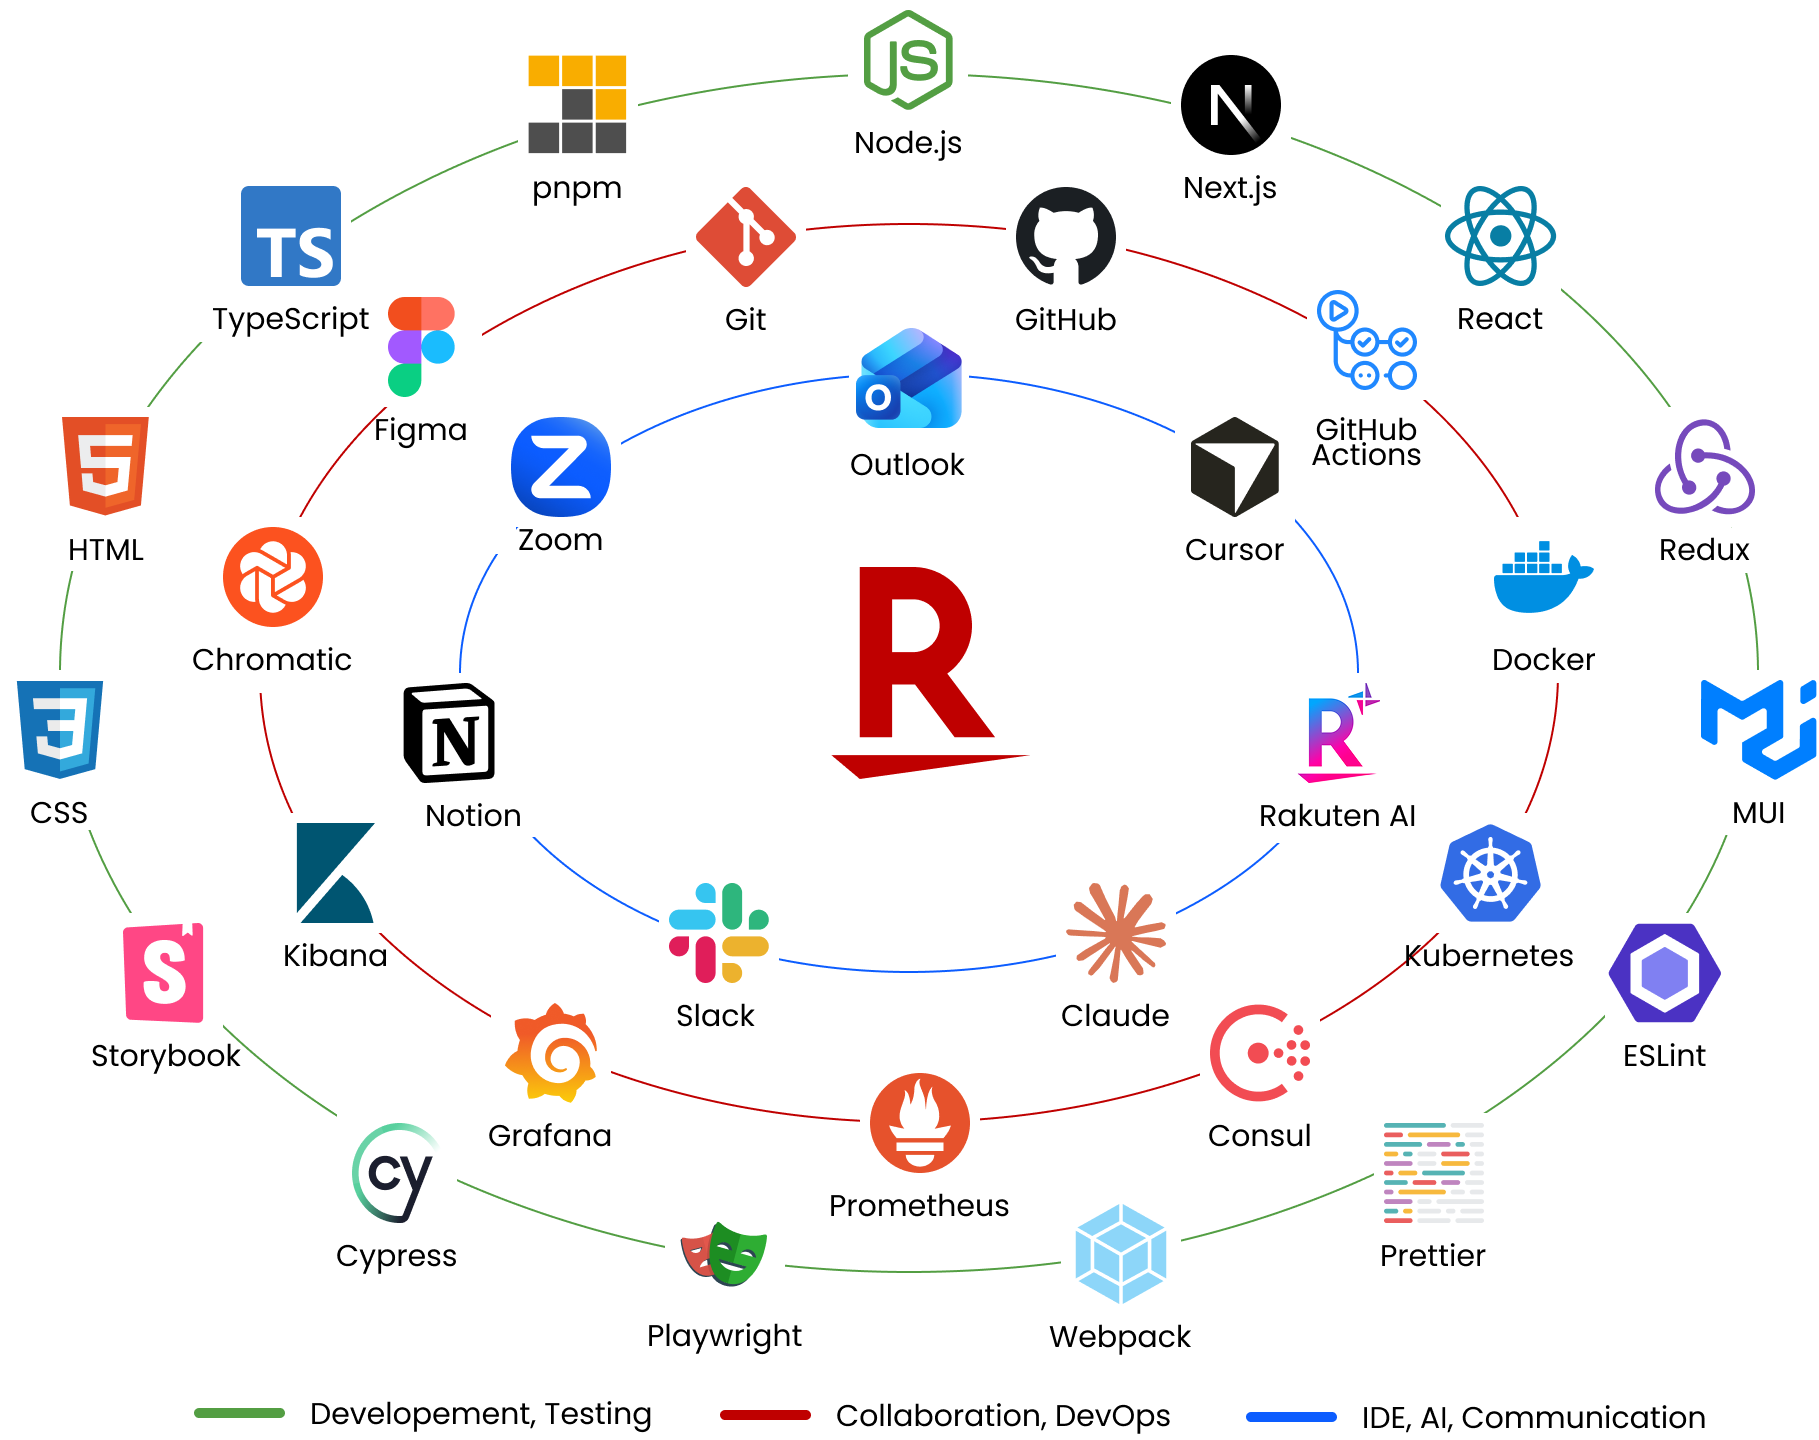
\includegraphics[width=\textwidth]{../assets/tools/rakuten_technical_environment.png}
    \caption{Rakuten France frontend technical ecosystem.}
    \label{fig:rakuten-technical-ecosystem}
\end{figure}

Figure~\ref{fig:rakuten-technical-ecosystem} illustrates the technical environment used by the frontend teams at Rakuten France, highlighting the key tools, frameworks, and practices that contribute to a streamlined development process.

\section{Development Languages and Frameworks}

The frontend applications are primarily developed using \textbf{\acs{HTML}}, \textbf{\acs{CSS}}, and \textbf{\acs{TS}}, which constitute the foundation of modern web development. \ac{TS} is preferred for its strong typing capabilities, improving code reliability, maintainability, and developer experience.

Rakuten France relies on \textbf{Next.js} as its primary frontend framework. Built on top of React, Next.js provides advanced features such as \textit{\ac{SSR}} and \textit{\ac{SSG}}, which improve application performance, \ac{SEO}, and \ac{UX}. \textbf{React} serves as the core library for building reusable and interactive \ac{UI}s, while \textbf{Redux} is employed for centralized state management, ensuring predictable application behavior and facilitating the management of complex application states.

Additionally, \textbf{\ac{MUI}} is used as a component library to accelerate frontend development by providing a collection of reusable, customizable, and accessible user interface components. It ensures design consistency across applications while reducing the time required to implement common interface elements.

The development environment is powered by \textbf{Node.js}, which provides the JavaScript runtime required for building and executing frontend applications. \textbf{Webpack} is used as the module bundler to efficiently compile and optimize application assets during development and production builds.

Dependency management is handled through \textbf{pnpm}, a fast and disk-efficient package manager that significantly reduces installation times while optimizing storage through content-addressable dependency sharing.

To organize the codebase, Rakuten France adopts a \textbf{monorepo} architecture managed with \textbf{Nx} and \textbf{Lerna}. This approach enables multiple frontend packages and shared components to coexist within a single repository, promoting code reuse, consistency, and simplified dependency management across features teams.

\section{Testing and Quality Assurance}

Maintaining high software quality is an essential aspect of the development process at Rakuten France. Several tools are integrated into the development workflow to ensure code quality, consistency, and application reliability.

\subsection{Code Quality}

\textbf{ESLint} is used to enforce coding standards and detect potential programming warnings and errors during development, while \textbf{Prettier} automatically formats source code according to predefined style guidelines. Together, these tools contribute to a clean, readable, and maintainable codebase.

\subsection{End-to-End Testing}

End-to-end testing is performed using both \textbf{Playwright} and \textbf{Cypress}, allowing developers to validate application behavior across different browsers and user interaction scenarios. These testing frameworks help identify regressions and ensure that critical business functionalities operate correctly before deployment.

\subsection{Component Development}

For component-driven development, \textbf{Storybook} is employed to develop, test, and document user interface components in isolation. This methodology encourages component reusability, simplifies \acs{UI} testing, and improves collaboration between developers and designers.

\section{Collaboration and Development Workflow}

Efficient collaboration is achieved through the use of \textbf{Git} as the distributed version control system. Git enables developers to work independently on different features while maintaining a complete history of code changes.

Source code hosting and project collaboration are managed through \textbf{GitHub}, which provides pull requests, code reviews, issue tracking, and continuous integration capabilities. These features support collaborative software development while ensuring code quality through peer review.

For browser-based development, testing, and debugging, \textbf{Chromium} is primarily used to verify application compatibility with modern web standards and to analyze application behavior during development.

\section{DevOps and Infrastructure}

To ensure reliable deployment, scalability, and monitoring of applications, Rakuten France relies on a set of DevOps tools and practices. These technologies automate development workflows, facilitate application delivery, and provide observability capabilities throughout the software lifecycle.

\textbf{GitHub Actions} is used to automate continuous integration and delivery workflows. It enables the execution of automated tasks such as code quality checks, testing, building applications, and deployment processes. This automation improves development efficiency and ensures consistent delivery pipelines.

\textbf{Docker} is used for containerization, allowing applications and their dependencies to be packaged into lightweight and portable containers. This approach ensures consistency between development, testing, and production environments while simplifying application deployment.

For container orchestration and scalability management, \textbf{\ac{K8S}} is adopted to automate the deployment, scaling, and management of containerized applications. It provides mechanisms for service discovery, load balancing, and fault tolerance, which are essential for maintaining reliable applications at scale.

Application monitoring and observability are supported through several dedicated tools. \textbf{Prometheus} is used for collecting and storing metrics, enabling real-time monitoring of application and infrastructure performance. \textbf{Grafana} is integrated with Prometheus to provide interactive dashboards and visualizations, allowing teams to analyze system health and identify potential issues.

\textbf{Kibana} is used for log analysis and visualization, providing insights into application behavior and facilitating troubleshooting. It works alongside the Elasticsearch ecosystem to centralize and explore application logs efficiently.

Finally, \textbf{Consul} is used for service discovery and configuration management. It enables communication between distributed services by providing service registration, health checking, and dynamic service discovery capabilities.

\section{Development Environment}

The primary \ac{IDE} adopted by the frontend teams is \textbf{Cursor}. Built upon \acf{VSCode}, Cursor provides a lightweight and highly customizable coding environment enriched with modern development features. Its extensive extension ecosystem, integrated debugging capabilities, and \acs{AI}-assisted functionalities significantly enhance developer productivity and streamline the software development process.

\section{Documentation and Project Management}

Documentation and project management are essential aspects of the development workflow at Rakuten France. \textbf{Notion} is used as a collaborative workspace for organizing technical documentation, managing tasks, and centralizing project-related information. It provides a unified platform where teams can create and maintain technical specifications, development guidelines, meeting notes, and knowledge bases.

Notion is also used for ticket management, allowing teams to track tasks, monitor progress, and maintain visibility over ongoing development activities. This approach facilitates knowledge sharing, improves team organization, and ensures that important project information remains accessible to all stakeholders.

\section{Communication}

Effective communication between distributed teams is supported through several collaboration tools. \textbf{Slack} is used as the primary instant messaging platform, enabling real-time discussions, team coordination, and quick information sharing between developers and other stakeholders.

\textbf{Outlook} is used for professional email communication, calendar management, and scheduling meetings. It ensures efficient coordination of activities across different teams and departments.

For online meetings and remote collaboration, \textbf{Zoom} is used to conduct virtual meetings, technical discussions, and team sessions. It provides reliable communication capabilities for distributed teams working across different locations.

\section{Artificial Intelligence Assistance}

\acf{AI} has become an integral part of the software development workflow at Rakuten France. Developers leverage \acs{AI}-powered tools to automate repetitive tasks, accelerate development, and improve code quality.

\textbf{Rakuten AI} is an internal \acs{AI} assistant designed to support software engineers in tasks such as code generation, documentation writing, code review, and technical assistance. By providing context-aware recommendations, it helps developers increase productivity while maintaining coding standards.

In addition, \textbf{Claude}, integrated directly into Cursor, assists developers through intelligent code completion, code explanation, refactoring suggestions, and documentation generation. The integration of \acs{AI} into the development environment reduces development time, facilitates knowledge sharing, and contributes to the overall quality and maintainability of software products.